\chapter{Elementi orbitali}
\label{chap:elementi-orbitali}

Nel precedente capitolo abbiamo determinato l'equazione
dell'orbita~\eqref{eq:orbita} che lega la coordinata polare $r$ all'altra
coordinata $\theta$, che dipende a sua volta dal tempo. La seconda legge di
Keplero, però, ci dice che $\theta$ non varia in maniera costante con il tempo,
eccetto nel caso particolare di orbita circolare. In questo capitolo ci
occuperemo della determinazione della posizione, in un dato istante di tempo,
della particella relativa che si muove su un'orbita ellittica.

\section{Equazione di Keplero}
\label{sec:equazione-keplero}

\begin{figure}
  \centering
  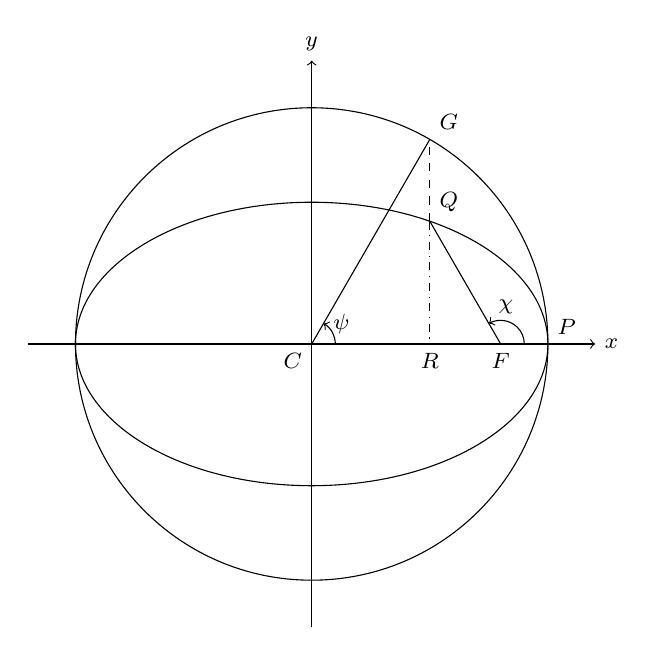
\begin{tikzpicture}[font=\footnotesize,scale=3]
    % a=1, e=0.8, b=a*sqrt(1-e^2)=0.6, c=ae=0.8, p=a*(1-e^2)=0.36, chi=120,
    % r(chi)=0.6, x_Q=x_G=c+r(chi)*cos(chi)=0.5,
    % y_Q=r(chi)*sin(chi)=0.5196, y_G=y_Q*a/b=0.866, psi=60 (deriva dalla relazione
    % fra anomalia vera ed eccentrica)
    \draw [->] (-1.2,0) -- (1.2,0) node[right] {$x$}; %asse x
    \draw [->] (0,-1.2) -- (0,1.2) node[above] {$y$}; %asse y
    \draw (0,0) circle (1); % circonferenza ausiliaria
    \draw (0,0) ellipse (1 and 0.6); %ellisse
    \draw (0.8,0) -- (0.5,0.5196) node[above right] {$Q$}; % segmento FQ
    \draw [dashed] (0.5,0.5196) -- (0.5,0.866); % segmento QG
    \draw (0,0) -- (0.5,0.866) node[above right] {$G$}; % segmento CG
    \draw (0,0) node[below left] {$C$}; % etichetta del punto C
    \draw (0.8,0) node[below] {$F$}; % etichetta del punto F
    \draw (1,0) node[above right] {$P$}; % etichetta del punto P
    \draw [dashdotted] (0.5,0.5196) -- (0.5,0) node[below] {$R$}; % segmento RQ
    \draw [->] (0.9,0) arc (0:120:0.1) node[above right] {$\chi$}; % angolo chi
    \draw [->] (0.1,0) arc (0:60:0.1) node[right] {$\psi$}; % angolo psi
  \end{tikzpicture}
  \caption[Ellisse e circonferenza ausiliaria per l'equazione di
  Keplero]{Ellisse e circonferenza ausiliaria concentrica. Abbiamo posto $a=1$
    ed $e=0.8$}
  \label{fig:circonferenza-ausiliaria-keplero}
\end{figure}
La seconda legge di Keplero permette di trovare la posizione relativa di un
corpo di un sistema binario in un qualsiasi istante di tempo. Con riferimento
alla figura~\ref{fig:circonferenza-ausiliaria-keplero}, il punto $Q$
dell'ellisse indica la posizione del corpo all'istante di tempo $t$ e $P$ la
posizione del periapside, da cui il corpo passa all'istante
$t_0$. Nell'intervallo di tempo $t-t_0$ il raggio vettore che congiunge il fuoco
$F$ alla posizione del corpo sull'ellisse si sposta da $FP$ a $FQ$, spazzando
dunque l'area $FPQ$. Allora per la seconda legge di Keplero
\begin{equation}
  \text{area } FPQ : \text{area ellisse} = t-t_0 : T,
\end{equation}
da cui otteniamo
\begin{equation}
  \text{area } FPQ = \frac{\pi ab(t-t_0)}{T}.
\end{equation}
Definendo la \emph{velocità angolare media} $\omega = 2\pi/T$ questa equazione
diventa
\begin{equation}
  \text{area } FPQ = \frac{1}{2}\omega ab(t-t_0).
\end{equation}
Conoscendo l'istante di passaggio al periapside $t_0$, il periodo di rivoluzione
$T$, il semiasse maggiore $a$ e l'eccentricità $e$, legata al semiasse minore
dalla~\eqref{eq:semiasse-minore-ellisse}, è possibile calcolare in un qualsiasi
istante di tempo $t$ l'area $FPQ$ da cui si ricava la posizione $Q$. Sebbene
questa tecnica sia molto semplice teoricamente, è poco utile nella pratica. Si
usa invece il metodo che ci apprestiamo a illustrare.

Circoscriviamo all'ellisse una circonferenza ausiliaria di raggio $a$ e
concentrica con l'ellisse, come nella
figura~\ref{fig:circonferenza-ausiliaria-keplero}.  Sia $G$ l'intersezione con
la circonferenza della perpendicolare all'asse $x$ innalzata dal punto
$Q$. L'angolo $G\widehat{C}P$, dove $C$ è il centro della circonferenza, è
chiamato \emph{anomalia eccentrica} e lo indicheremo con $\psi$. Al periapside
si ha $\chi = \psi = 0$ e all'apoapside $\chi = \psi = \pi$. I punti
$Q=(x_Q,y_Q)$ e $G=(x_Q,y_G)$ hanno la stessa ascissa e vogliamo trovare una
relazione fra le loro ordinate. Per fare questo ricordiamo che l'equazione
cartesiana di una circonferenza di raggio $a$ e centro l'origine del sistema di
riferimento è
\begin{equation}
  x_\textup{c}^2 + y_\textup{c}^2 = a^2.
\end{equation}
Invece, l'equazione di un'ellisse con centro nell'origine del sistema e semiassi
maggiore $a$, lungo l'asse $x_\textup{e}$, e minore $b$, lungo l'asse
$y_\textup{e}$, è
\begin{equation}
    \frac{x_\textup{e}^2}{a^2} + \frac{y_\textup{e}^2}{b^2} = 1.
\end{equation}
Se gli assi dei sistemi di riferimento delle due coniche sono coincidenti,
uguagliando le ascisse risulta
\begin{equation}
  x_\textup{c}^2 = x_\textup{e}^2 \iff a^2 - y_\textup{c}^2 = a^2 -
  y_\textup{e}^2a^2/b^2 \iff \abs{y_\textup{c}} = \abs{y_\textup{e}}a/b.
\end{equation}
Allora, per i punti $Q$ e $G$ abbiamo che $y_G = y_Qa/b$. D'altra parte,
$y_Q = r\sin\chi$ e $y_G = a\sin\psi$, cioè
\begin{equation}
  \label{eq:r-sin-chi}
  r\sin\chi = b\sin\psi.
\end{equation}
Inoltre $\overline{FR} =
r\cos\chi$,\footnote{Un
  valore negativo di $\overline{FR}$ indica che il punto $R$ si trova alla
  sinistra di $F$ sull'asse $x$.} ma è anche $\overline{FR} = \overline{CR} -
\overline{CF} = a\cos\psi - ae$, da cui
\begin{equation}
  \label{eq:r-cos-chi}
  r\cos\chi = a(\cos\psi - e).
\end{equation}
Sommando membro a membro i quadrati delle equazioni~\eqref{eq:r-sin-chi}
e~\eqref{eq:r-cos-chi} otteniamo
\begin{equation}
  \begin{split}
    r^2 &= r^2\cos^2\chi + r^2\sin^2\chi = a^2(\cos\psi - e)^2 + b^2\sin^2\psi\\
    &= a^2\cos^2\psi-2a^2e\cos\psi+a^2e^2+a^2\sin^2\psi-a^2e^2\sin^2\psi\\
    &= a^2(1+e^2-2e\cos\psi-e^2\sin^2\psi) = a^2(1-2e\cos\psi+e^2\cos^2\psi)\\
    &= a^2(1 - e\cos\psi)^2,
  \end{split}
\end{equation}
da cui ricaviamo la seguente equazione che lega la coordinata polare $r$ con
l'anomalia eccentrica $\psi$
\begin{equation}
  \label{eq:r-anomalia-eccentrica}
  r = a(1 - e\cos\psi).
\end{equation}
Dall'equazione~\eqref{eq:terza-legge-keplero} che esprime la terza legge di
Keplero
\begin{equation}
  \omega^2 = \frac{4\pi^2}{T^2} = \frac{GM_\textup{T}}{a^3}.
\end{equation}
Ricordando la~\eqref{eq:reciproco-semilato}, la~\eqref{eq:semilato-ellisse} e
la~\eqref{eq:velocita-tangenziale} abbiamo
\begin{equation}
  \begin{split}
    r^2\dot{\chi}^2 &= \frac{l_0^2}{\mu^2p^2}(1 + e\cos\chi)^2 =
    \frac{l_0^2}{\mu^2p} \frac{(1+e\cos\chi)^2}{a(1-e^2)} \\
    &= GM_\textup{T} \frac{(1+e\cos\chi)^2}{a(1-e^2)} = \omega^2a^3
    \frac{(1+e\cos\chi)^2}{a(1-e^2)} \\
    &= \omega^2a^4 \frac{(1+e\cos\chi)^2}{a^2(1-e^2)^2}(1-e^2) =
    \frac{\omega^2a^4(1-e^2)}{r^2}.
  \end{split}
\end{equation}
Quindi, dalla~\eqref{eq:velocita-ellisse}, il quadrato della derivata temporale
di $r$ è
\begin{equation}
  \begin{split}
    \dot{r}^2 &= v^2 - r^2\dot{\chi}^2 = GM_\textup{T}
    \left(
      \frac{2}{r} - \frac{1}{a}
    \right) - \frac{\omega^2a^4(1-e^2)}{r^2} \\
        &= \omega^2a^3
    \left(
      \frac{2}{r} - \frac{1}{a}
    \right) - \frac{\omega^2a^4(1-e^2)}{r^2} \\
    &= \frac{2\omega^2a^3r-r^2\omega^2a^2-\omega^2a^4+\omega^2a^4e^2}{r^2}\\
    &= \frac{\omega^2a^2}{r^2}(a^2e^2-(r-a)^2)
  \end{split}
\end{equation}
da cui
\begin{equation}
  \toder{r}{t} = \dot{r} = \frac{\omega a}{r}\sqrt{a^2e^2 - (r-a)^2}.
\end{equation}
Per risolvere questa equazione differenziale ordinaria cambiamo la funzione
incognita da $r$ in $\psi$ effettuando la
sostituzione~\eqref{eq:r-anomalia-eccentrica}. Deriviamo
la~\eqref{eq:r-anomalia-eccentrica} rispetto al tempo
\begin{equation}
  \dot{r} = ae\dot{\psi}\sin\psi.
\end{equation}
Sostituiamo la~\eqref{eq:r-anomalia-eccentrica} nell'equazione differenziale
\begin{equation}
  r = \frac{\omega a\sqrt{a^2e^2 - a^2e^2\cos^2\psi}}{a(1-e\cos\psi)} =
  \frac{\omega ae\sin\psi}{1-e\cos\psi}.
\end{equation}
Uguagliando le due espressioni di $\dot{r}$ così ottenute ricaviamo
\begin{equation}
  \toder{\psi}{t} = \dot{\psi} = \frac{\omega}{1-e\cos\psi}.
\end{equation}
Ricordando che al perielio abbiamo $t = t_0$ e $\psi = 0$, integriamo questa
equazione differenziale fino a un generico istante di tempo $t$ in cui
l'anomalia eccentrica vale $\psi$
\begin{gather}
  \int_{t_0}^t \omega\dd \tau = \int_0^\psi(1-e\cos\psi')\dd \psi' \iff\\
  \phi = \omega(t - t_0) = \psi - e\sin\psi, \label{eq:keplero}
\end{gather}
dove $\phi = \omega(t-t_0)$ è chiamata \emph{anomalia media}. Questa equazione è
detta \emph{equazione di Keplero}. In ogni fissato istante di tempo $t$, la sua
soluzione $\psi$ permette di ricavare, tramite
la~\eqref{eq:r-anomalia-eccentrica}, la coordinata polare $r$. Inoltre possiamo
determinare una relazione tra l'anomalia eccentrica e l'altra coordinata polare
$\chi$. Infatti, uguagliando i secondi membri delle equazioni~\eqref{eq:orbita}
e~\eqref{eq:r-anomalia-eccentrica} abbiamo
\begin{equation}
  \begin{aligned}
    a(1-e\cos\psi) &= \frac{a(1-e^2)}{1+e\cos\chi} \iff 1+e\cos\chi =
    \frac{1-e^2}{1-e\cos\psi} \iff \\
    e\cos\psi &= \frac{1-e^2-1+e\cos\psi}{1-e\cos\psi} =
    \frac{e(\cos\psi-e)}{1-e\cos\psi} \iff \\
    \cos\psi &= \frac{\cos\psi-e}{1-e\cos\psi}.
  \end{aligned}
\end{equation}
Aggiungiamo e sottraiamo ambo i membri dell'ultima equazione da $1$
\begin{align}
  \begin{split}
    1-\cos\chi &= 1-\frac{\cos\psi-e}{1-e\cos\psi} =
    \frac{1-e\cos\psi-\cos\psi+e}{1-e\cos\psi} \\
    &= \frac{(1+e)(1-\cos\psi)}{1-e\cos\psi}
  \end{split} \\
  \begin{split}
    1+\cos\chi &= 1+\frac{\cos\psi-e}{1-e\cos\psi} =
    \frac{1-e\cos\psi+\cos\psi-e}{1-e\cos\psi} \\
    &= \frac{(1-e)(1+\cos\psi)}{1-e\cos\psi}.
  \end{split}
\end{align}
Facendo il rapporto dei primi e ultimi membri di queste equazioni troviamo
la relazione cercata
\begin{gather}
  \frac{1-\cos\chi}{1+\cos\chi} = \frac{1+e}{1-e}\frac{1-\cos\psi}{1+\cos\psi}
  \iff \\
  \tan^2\frac{\chi}{2} = \frac{1+e}{1-e}\tan^2\frac{\psi}{2}.
\end{gather}

\section{Soluzioni dell'equazione di Keplero}
\label{sec:soluzioni}

L'equazione di Keplero~\eqref{eq:keplero} è trascendente nell'incognita $\psi$
per via del termine $\sin\psi$, e non ammette soluzione analitica, ma possono
essere utilizzati diversi metodi numerici per risolverla.

\subsection{Metodo di Newton~-~Raphson}
\label{sec:newton}

\subsection{Integrali ellittici}
\label{sec:integrali-ellittici}

\subsection{Funzioni di Bessel}
\label{sec:bessel}

%%% Local Variables:
%%% mode: latex
%%% TeX-master: "../tesi"
%%% End:
